\documentclass[a4paper]{article}
\usepackage{geometry}
\geometry{total={170mm,250mm}, top=25mm}

\usepackage{graphicx} % Required for inserting images
\usepackage{amsmath}
\date{}
\usepackage[utf8]{inputenc}
\usepackage{fancyhdr}
\usepackage{algorithm}
\usepackage{algpseudocode}
\title{Shannon's Mind Reading Game}
\usepackage[toc,page]{appendix}
\DeclareMathOperator*{\Index}{\textbf{Index}}
\fancyhf{}
\fancyhead[L]{Bachelors of Statistics (Hons.), 2023-26}
\fancyfoot[R]{Shannon's Trick}
\fancyfoot[C]{\thepage}
\fancyfoot[L]{Statistical Methods - I}
\setlength{\headsep}{35pt}
\renewcommand{\footrule}{
        \hrule width\headwidth height\headrulewidth depth\headrulewidth
}

\usepackage{enumitem}

\newcommand{\definition}[2]{%
    \begin{minipage}{\textwidth}
        \textbf{#1:} #2
    \end{minipage}
    % \begin{itemize}[label=\textbullet, leftmargin=*]
}

% \newcommand{\defitem}[1]{%
%     \item #1
% }

% \newcommand{\enddefinition}{%
%     \end{itemize}
% }


%%%%%%%%%%%%%%%%%%%%%% stuff
% to do: what happens for more than three riffle shuffles?

\begin{document}
\input{title/title.tex}
\pagestyle{fancy}
\maketitle
\author{}
\date{}
\begin{abstract}
    Claude Shannon, famously known as the father of 
    information theory, is credited with inventing this magic trick.
    We characterize the setup, and then implement the algorithm 
    used by Claude Shannon. To do this, 
    we appropriately choose the models which represent the 
    transitions. This project empirically confirms the success of this
    trick.
\end{abstract}
\section{Problem Statement}
\textbf{Magician} and \textbf{User} play a game. The \textbf{Magician} \textbf{riffle shuffles} an ordinary deck thrice, and sends it to the \textbf{User}.
\textbf{User} picks a card from the top, and then inserts 
it back into the deck randomly. The \textbf{User} sends the deck back to the \textbf{Magician}: who finds out 
the picked card.
\begin{center}
    \includegraphics*[width=500pt]{files/Setup.jpg}
\end{center}
\newpage
\section{Setup}
\begin{itemize}
    \item Pick a bijection $$\Psi:\textbf{Deck} \to \{1, 2, \cdots, 52\}$$ We 
    henceforth only talk about $\{1, 2, \cdots, 52\}$, as the algorithm used doesn't
    depend on the specific type of the card in consideration. 
    \item \textbf{Riffle Shuffle:} A specific method of shuffling cards by 
    dividing a deck into roughly equal halves, and then interweaving the two 
    halves by successively interleaving the cards from each half, in a randomized
    order. 
    \item Any arrangement of the $\Psi(\textbf{Deck})$ is a permutation of $[52]$. 
    Consider any permutation $\sigma$, we define 
    $$\Index(\sigma) = \{\sigma(1), \sigma(2), \cdots, \sigma(52)\}$$
    \item \textbf{Rising Sequence:} Given a permutation $\sigma$, $S_a = \{a, a+1, \cdots, a + k -1\} \subseteq \sigma(\Psi(\textbf{Deck}))$ is
    called a rising sequence of size $k$ if $$\sigma(a-1) \not< \sigma(a) < \sigma(a+1) < \cdots < \sigma(a+k-1) \not< \sigma(a+k)$$ 
\end{itemize}
\section{Idea}
The idea is to notice that the final deck has a unique Rising Sequence of size $1$
pretty often. 
\newline 
To implement this, we would have to fix appropriate models for the steps involved: 
splitting the decks, interweaving them, randomly putting the card in at some index. 
The models we use are: 
\begin{itemize}
    \item $\textbf{Deck splitting:}$ We split a deck $100$ times and counted the size of the smaller deck. 
    Then, we flipped a coin for each entry $x$ and picked $x$ or $52 - x$ randomly, in the final dataset, to ensure
    there are no \textbf{IID} issues. Atlast, we fit a normal distribution over this dataset to get: 
    $$\mathcal{N}(\mu, \sigma^2) = \mathcal{N}(25.78, 2.3046^2)$$
    \item $\textbf{Interweaving them:}$ We maintain two arrays \textbf{Right}, \textbf{Left}. The probability that 
    the next card falls from the $\textbf{Right}$ is $\dfrac{|\textbf{Right}|}{|\textbf{Right}| + |\textbf{Left}|}$ and 
    from the \textbf{Left} is  $\dfrac{|\textbf{Left}|}{|\textbf{Right}| + |\textbf{Left}|}$. This is justified by drawing from domain knowledge 
    that the weights of the hands are linearly related to the number of cards.
    \item $\textbf{Randomly putting it in somewhere:}$ We use $\text{Binom}(52, \frac{1}{2})$, as humans are, probably, more likely
    to put the card somewhere close to the middle.
\end{itemize}  
\newpage
\section{Implementation}
The following algorithms were used in the project. 
\begin{algorithm}
\caption{ Riffle Shuffle the deck of cards}\label{riffle}
\begin{algorithmic}[1]
\Procedure{RiffleShuffle}{Cards}
    \State \textbf{Deck} $:= \{\}$
    \State \textbf{split} $ := \operatorname{\textbf{floor}}(\operatorname{\textbf{rnorm}}(1, \text{\textbf{mean}} = 25.78, \text{\textbf{sd}} = 2.3046))$

    \State \textbf{LeftHand} $:= \text{Cards}[1:\textbf{split}]$
    \State \textbf{RightHand} $:= \text{Cards}[\textbf{split}+1: 52]$ 
    \For{$i$ in $\{1, 2, \cdots, 52\}$ }
    \State \textbf{hand} $:= \text{sample}((L,R), \text{prob}=(\text{size}(\textbf{LeftHand}), \text{size}(\textbf{RightHand})))$\Comment{hand the Card falls from}
    \If{\textbf{hand} $== L$ }
    \State \textbf{Deck} $\leftarrow \textbf{LeftHand}[1]$
    \State \text{pop}(\textbf{LeftHand})\Comment{remove the added Card}
    \Else 
    \State \textbf{Deck} $\leftarrow \textbf{RightHand}[1]$
    \State \text{pop}(\textbf{RightHand})
    \EndIf
    \EndFor

    \State \textbf{return Deck}
\EndProcedure
\end{algorithmic}
\end{algorithm}
\begin{algorithm}
\caption{ Count number of Rising Sequences of size $1$ and check if it's unique}\label{risingseq}
\begin{algorithmic}[1]
\Procedure{RisingSingleton}{$S$}
    \State $\Index := \{\}$
    \For{$i$ in $\{1, 2, \cdots 52\}$}
    \State $\Index[S[i]] = i$\Comment{Define the $\Index$ array.}
    \EndFor
    \State $\textbf{Sum} := 0, \textbf{ SingletonCard} := 0$
    \For{$i$ in $\{1, 2, \cdots, 52\}$}
    \If{$\Index[i] \geq \Index[i+1] \text{ and } \Index[i] \leq \Index[i-1]$}\Comment{Singleton Rising Sequence}
    \State $\textbf{Sum} = \textbf{Sum} + 1$
    \State $\textbf{SingletonCard} = i$
    \EndIf
    \EndFor
    \State $\textbf{return } (\textbf{Sum} == 1), \textbf{ SingletonCard}$
\EndProcedure
\end{algorithmic}
\end{algorithm}
\newpage
\section{Experimental Setup}
The code simulates the magician's guessing by repeating the process 10,000 times.
\begin{itemize}
    \item A deck of cards, numbered 1 to 52 in ascending order, is defined.
    \item The \texttt{RiffleShuffle} function is called three times, shuffling the original
deck.
\item The \texttt{Switch} function is used to place the top card somewhere
within the deck.
\item The \texttt{RisingSingleton} function identifies a potential unique rising sequence, and the count of unique singleton rising sequences is recorded.

\end{itemize}

\section{ Results and Conclusion}
The success percentage of \boxed{\textbf{91\%}}, calculated as the ratio of unique single rising sequence, which match the picked card, to the total attempts, indicates the probability of identifying
the top card. This percentage demonstrates the effectiveness of the method in
predicting the chosen card in a card guessing scenario.\newline
\newline 
\section{Beyond}

The setup had us pick the $\textif{first}$ card. However, playing with the index where the card is picked from is something interesting. 
We did this, and calculated the success percentage for all possible starting indexes $(\sim 5200000$ trials$)$
This results in an interesting graph attached in the next page.  
\begin{figure}. 
    \centering
    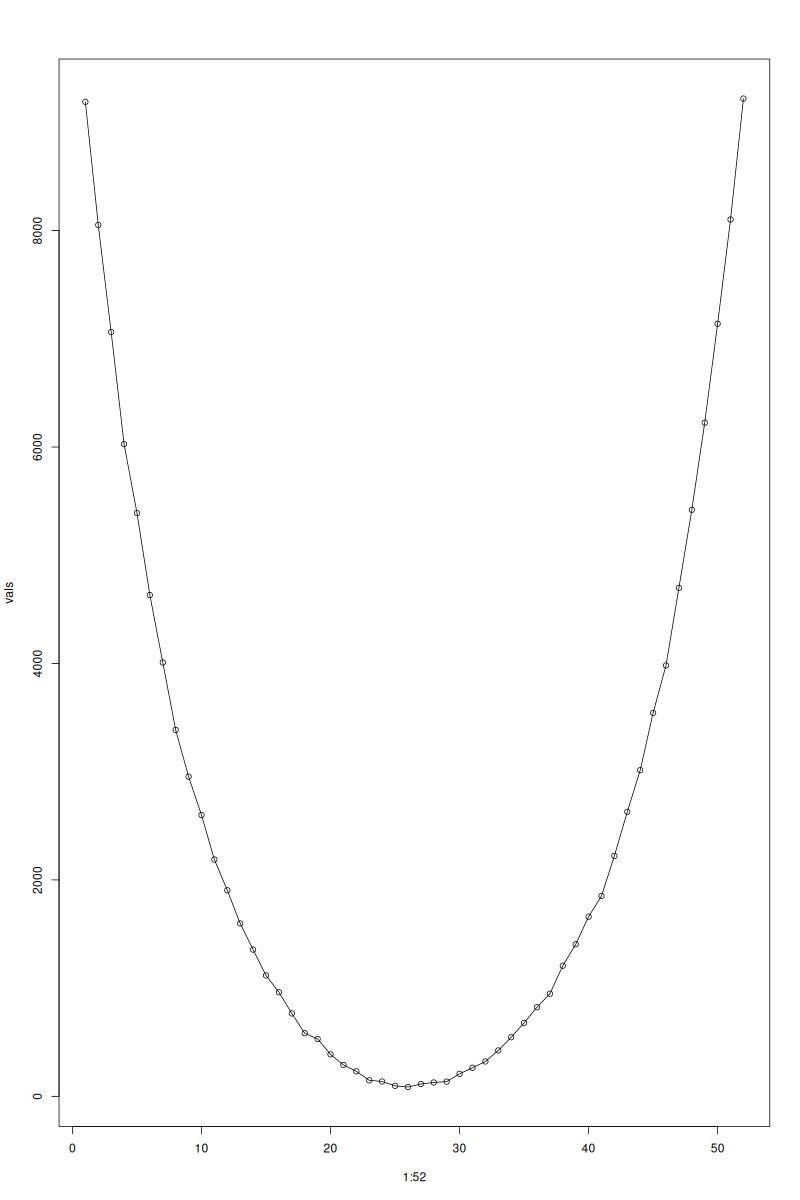
\includegraphics[width=\linewidth ]{graph.jpeg}
\end{figure}

\end{document}
